\documentclass{scrartcl}

\usepackage{fullpage}
\usepackage[utf8]{inputenc}
\usepackage{hyperref}
\usepackage{float}
\usepackage{verbatim}
\usepackage{color}
\usepackage{tikz}
\usetikzlibrary{positioning, shapes, arrows}

\title{Report Generator}
\subtitle{module for otu.lea}
\author{Tamás Nagy\\ \small nattomi@gmail.com}

\begin{document}
\maketitle
\tableofcontents
\section{Introduction}
\href{http://github.com/nattomi/otulear}{Report Generator} is a module of the more complex \href{http://workforce.zmml.uni-bremen.de}{otu.lea} project. It is used for generating plain text and pdf reports about the performance of the users of the main \href{http://www.ifeb.uni-bremen.de/otulea/reaApplication.html}{otulea} test-taking application. It is a collection of \href{http://github.com/nattomi/otulear/tree/master/scripts}{scripts} (written in R and PHP) and \LaTeX\ templates. Additionally, routines used in the above mentioned scripts are also wrapped into an \href{http://github.com/nattomi/otulear/tree/master/otulea}{R package}. Momentarily it is not clear weather the R package is of any use, so its develepment is inactive. 

\section{How report generation works?}
Report generation is a process consisting of the following steps:
\begin{enumerate}
\item Load content of input data sources (such as .xml files) into memory
\item Extract information to be reported
\item\label{organ} Organize information to be reported into a structured form (such as .xml or .tex files)
\item If needed, run an external program (such as pdflatex) to translate the output of \ref{organ} into a human-readable form. 
\end{enumerate}
\begin{figure}[t]
\begin{center}
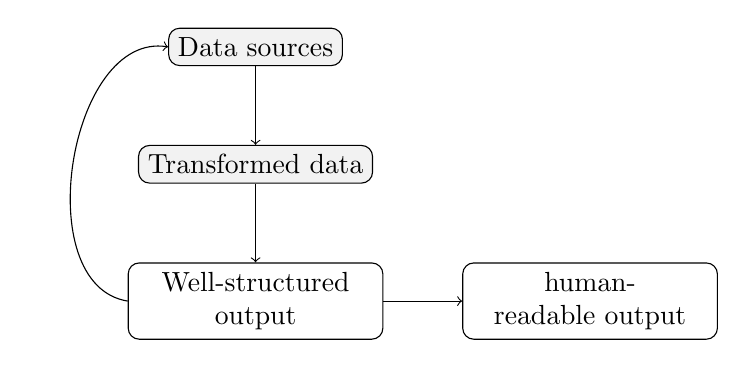
\begin{tikzpicture}[
mynode/.style={draw,fill=gray!10,rounded corners,align=center},
output/.style={draw,rounded corners,align=center}
]
\node[mynode] (sources) at (0,0) {Data sources};
\node[mynode, below=of sources] (trans) {Transformed data};
\node[output, below=of trans,text width=3cm] (struct) {Well-structured output};
\node[output,right=of struct,text width=3cm] (human) {human-readable output};
\draw[->] (sources) -- (trans);
\draw[->] (trans) -- (struct);
\draw[->] (struct) -- (human);
\path[->] (struct) edge [bend left=90] (sources);
\end{tikzpicture}
\end{center}
\caption{Simplified flow chart of report generation. It might be the case that a well-structured output of the report generation process becomes an input data source in a later stage.
}
\end{figure}
As an example, let's consider a speacial way to interpret the data generated by users of the otu.lea system, the so-called \emph{student report}. Here, we load certain .xml files, do some calculations on them according to some rules and dump the results of our calculations as an .xml file again. This .xml file is already an becomes the input of a new calculation stream which outputs a .tex file. This file is then rendered into a pdf file using pdflatex. We talk about this later in more detail.

In general, we can say that there is always some sort of database (either a relational one our a database of static files in a well-organized folder hierarchy just like in the case of otu.lea) we get our data from. We can think of report generation as if it were a certain \emph{view} to our database -- similar to the concept under the same name in database theory.

\section{The otu.lea database}
The database behind the otu.lea system is a collection of static .xml files. There are two main parts of this database. Files in the first part are for configuration purposes that only administrators can modify. From these, Report Generator only uses one file named \emph{alphalist.xml}. Files in the other part of the database are generated while users of the system are taking test-sessions. We use the term \emph{user files} to describe them.
\subsection{The alphalist.xml file}
\begin{figure}
\begin{center}
\begin{tikzpicture}[
mynode/.style={draw,fill=gray!10,rounded corners,align=center},
output/.style={draw,rounded corners,align=center,anchor=north}
]
\node[mynode] (root) at (0,0) {alphalist};
\node[output,anchor=north] (a1) at (-5,-1) {\parbox{2.6cm}{\textbf{alphanode}\\
\small{$\bullet$ alphaID\\
$\bullet$ order\\
$\bullet$ description\\
$\bullet$ userdescription\\
$\bullet$ example}}};
\node[output] (a2) at (-.5,-1) {\textbf{alphanode}};
\node[anchor=north] (a3) at (1.25,-1.1) {$\ldots$};
\node[output] (a4) at (3,-1) {\textbf{alphanode}};
\draw[--] (root) -- (a1);
\draw[--] (root) -- (a2);
\draw[--] (root) -- (a4);
\end{tikzpicture}
\end{center}
\caption{Tree structure of the alphalist.xml file. Each alphanode entry has 5 attributes.}
\label{fig:alphalist}
\end{figure}
The structure of the file is explained in Figure \ref{fig:alphalist}. It consists of multiple alphanode nodes. Each alphanode node has 5 attributes:
\begin{description}
\item[alphaID]: ability description ID.
\item[order]: unrelevant for Report Generator.
\item[description]: ability description displayed for teachers
\item[userdescription]: ability description displayed for students 
\item[example]: example clarifying ability description (to be shown to students)
\end{description}
Here is a snippet from the file:
\begin{verbatim}
<alphalist lang="german">
  <alphanode alphaID="1.2.1.2" order="60"
             description="Kann Zeitpläne sinnentnehmend lesen" 
             userdescription="Ich kann Zeitpläne lesen" example=""/>
 <alphanode alphaID="1.2.1.1" order="50" 
            description="Kann Wörter mit ansteigender Komplexität 
                        (Konsonantenhäufung) recodieren und decodieren" 
            userdescription="Ich kann einfache Wörter erkennen und lesen" 
            example=""/>
\end{verbatim}
\quad$\vdots$
\subsection{The user files}\label{subsection:userfiles}
There are two type of users of the otu.lea system: teachers and students. In this document -- if not otherwise stated -- by the term user we always mean students. Each user has an id which is a character string of a fixed length. Let's denote it by \verb+$userid+. Each user has a folder in the database named as \verb+$userid+. In each folder, there is a special file named \verb+$userid . ".xml"+ (we use the operator . for string concatenation as in PHP). This file describes the tests taken by the user, we call it the \emph{global user file}. It serves as a search index for finding the information related to any particular test a user has taken. From it we can determine:
\begin{itemize}
\item The date and time a partical test session was started
\item The subject and level of this particular test
\item The tasks contained by this particular test and the \emph{task-result files} linked to them
\end{itemize}
\begin{figure}
\begin{center}
\begin{tikzpicture}[
mynode/.style={draw,fill=gray!10,rounded corners,align=center},
output/.style={draw,rounded corners,align=center,anchor=north}
]
\node[mynode] (root) at (0,0) {performedtests};
\node[output,anchor=north] (a1) at (-5,-1) {\parbox{2.6cm}{\textbf{test}\\
\small{$\bullet$ timestamp\\
$\bullet$ subject\\
$\bullet$ level}}};
\node[output] (a2) at (-.5,-1) {\textbf{test}};
\node[anchor=north] (a3) at (1.25,-1.1) {$\ldots$};
\node[output] (a4) at (3,-1) {\textbf{test}};
\draw[--] (root) -- (a1);
\draw[--] (root) -- (a2);
\draw[--] (root) -- (a4);
\node[output,anchor=north] (i1) at (-10,-4) {\parbox{2.6cm}{\textbf{item}\\
\small{$\bullet$ iname\\
$\bullet$ data}}};
\node[output] (i2) at (-5.5,-4) {\textbf{item}};
\node[anchor=north] (i3) at (-3.75,-4.1) {$\ldots$};
\node[output] (i4) at (-2,-4) {\textbf{item}};
\draw[--] (a1) -- (i1);
\draw[--] (a1) -- (i2);
\draw[--] (a1) -- (i4);
\end{tikzpicture}
\end{center}
\caption{Tree structure of the global user file. It contains information about the performed tests and the tasks within those tests.}
\label{fig:guf}
\end{figure}
Figure \ref{fig:guf} shows the tree structure of the global user file. The main document consists of various \emph{test} nodes. Each test node has the follwing attributes:
\begin{description}
\item[timestamp] character string describing the date and time of the beginning of the test-session in the form of \verb+%Y_%m_%d_%H_%M_%S+ (see Appendix \ref{app:posix} for notation).
\item[subject] character string describing the subject of the test. It can be one of ``Lesen'', ``Schreiben'', ``Sprache'', ``Mathe''.
\item[level] character string describing the difficulty of the test. It can be one of ``Einfach'', ``Mittel'' and ``Schwer''. 
\end{description}
Furthermore, each test node has child nodes called \emph{item}. The attributes of each of these item nodes are in one-to-one correspondence with a task of the test the parent node referring to. It has the following attributes:
\begin{description}
\item[iname] character string describing the number of the task. The numbering convention of the tasks is not detailed here.
\item[data] character string describing the name of the task-result file. The task-result files of a user are located in the same folder as the global user file. 
\end{description}
Below is a snippet from a global user file:
\begin{verbatim}  
<performedtests>
  <test timestamp="2014_2_27_12_40_49" subject="Schreiben" level="Einfach">
    <item iname="2.1.01" data="KFCG1_2014_2_27_12_40_49_2.1.01.xml"/>
    <item iname="2.1.02_I" data="KFCG1_2014_2_27_12_43_37_2.1.02_I.xml"/>
    <item iname="2.1.02_II" data="KFCG1_2014_2_27_12_47_9_2.1.02_II.xml"/>
    <item iname="2.2.01_III" data="KFCG1_2014_2_27_12_48_53_2.2.01_III.xml"/>
    <item iname="2.2.02_I" data="KFCG1_2014_2_27_12_52_11_2.2.02_I.xml"/>
  </test>
  <test timestamp="2014_2_27_18_37_23" subject="Lesen" level="Mittel">
    <item iname="1.3.2" data="KFCG1_2014_2_27_18_37_23_1.3.2.xml"/>
    <item iname="1.3.3" data="KFCG1_2014_2_27_18_40_45_1.3.3.xml"/>
    <item iname="1.3.4" data="KFCG1_2014_2_27_18_42_27_1.3.4.xml"/>
    <item iname="1.3.6" data="KFCG1_2014_2_27_18_43_53_1.3.6.xml"/>
    <item iname="1.4.1" data="KFCG1_2014_2_27_19_11_28_1.4.1.xml"/>
    <item iname="1.4.2" data="KFCG1_2014_2_27_19_14_19_1.4.2.xml"/>
    <item iname="1.4.4" data="KFCG1_2014_2_27_19_18_7_1.4.4.xml"/>
    <item iname="1.4.5" data="KFCG1_2014_2_27_19_22_52_1.4.5.xml"/>
    <item iname="1.4.6" data="KFCG1_2014_2_27_19_25_18_1.4.6.xml"/>
    <item iname="1.4.7" data="KFCG1_2014_2_27_19_27_16_1.4.7.xml"/>
    <item iname="1.4.8" data="KFCG1_2014_2_27_19_29_40_1.4.8.xml"/>
  </test>
\end{verbatim}
\quad$\vdots$

The structure of the task-result files are more diverse, but as Report Generator only uses a specific segment of the file, we intruduce only this segment in Figure \ref{fig:taskresult}.
\begin{figure}
\begin{center}
\begin{tikzpicture}[
mynode/.style={draw,fill=gray!10,rounded corners,align=center},
output/.style={draw,rounded corners,align=center,anchor=north}
]
\node[mynode] (root) at (0,0) {item};
\node[output] (marking) at (0,-1) {marking};
\node[output] (pointuse) at (-7,-2.5) {pointuse};
\node[output] (m1) at (-3.5,-2.5) {\parbox{2.6cm}{\textbf{mark}\\
\small{$\bullet$ itemnumber\\
$\bullet$ alphalevel}}};
\node[output] (m2) at (-.5,-2.5) {\textbf{mark}};
\node at (.75,-2.75) {$\ldots$};
\node[output] (m3) at (2,-2.5) {\textbf{mark}};
\draw[--] (root) -- (marking);
\draw[--] (marking) -- (pointuse);
\draw[--] (marking) -- (m1);
\draw[--] (marking) -- (m2);
\draw[--] (marking) -- (m3);
\end{tikzpicture}
\end{center}
\caption{Tree structure of the segment of the task-result file relevant to Report Generator.}
\label{fig:taskresult}
\end{figure}
In the task-result files there is always a \emph{marking} node whose children nodes we are interested in. It always has a child node named \emph{pointuse} which is not relevant to our calculations so we omit describing it. Its other children nodes are all named \emph{mark} and they describe the performance of the user on a subtask of the task in question. Performance can be either 1 (passed) or 0 (failed). Each mark node has (at least) the following attributes:
\begin{description}
\item[itemnumber] character string describing the subtask number the mark node is referring to
\item[alphalevel] ability description id of the ability description which is tested by the mark node
\end{description} 
Below is the simplified version of a the task-result file showing only the nodes relevant to Report Generator.
\begin{verbatim}
<item>
  <marking>
    <pointuse maxpoint="1"/>
    <mark itemnumber="2.1.01_1a" alphalevel="2.1.05">1</mark>
    <mark itemnumber="2.1.01_1b" alphalevel="2.1.14">1</mark>
    <mark itemnumber="2.1.01_2a" alphalevel="2.1.05">1</mark>
    <mark itemnumber="2.1.01_2b" alphalevel="2.1.14">1</mark>
    <mark itemnumber="2.1.01_3a" alphalevel="2.1.05">1</mark>
    <mark itemnumber="2.1.01_3b" alphalevel="2.1.04">1</mark>
    <mark itemnumber="2.1.01_4a" alphalevel="2.1.05">1</mark>
    <mark itemnumber="2.1.01_4b" alphalevel="2.1.14">1</mark>
    <mark itemnumber="2.1.01_5a" alphalevel="2.1.05">1</mark>
    <mark itemnumber="2.1.01_5b" alphalevel="2.1.14">0</mark>
    <mark itemnumber="2.1.01_5c" alphalevel="2.1.14">0</mark>
  </marking>
</item>
\end{verbatim}

\section{Implementation of evalUser.R}
They are all located in the folder named s
\subsection{Introduction and basic usage examples}
This script is used for evaluating a user's performance. One can get the following help page by issuing \verb+./evalUser.R -h+:
\begin{verbatim}
Usage: ./evalUser.R [options]

Options:
	-u USER, --user=USER
		user id

	-t THRESHOLD, --threshold=THRESHOLD
		threshold for fullfilling a competency [defaults to 100]

	-m MAXLISTINGS, --maxlistings=MAXLISTINGS
		max. number of listings in order to limit the output to a fixed set of reported 
competencies or needs for improvement [defaults to  3]

	-T TIMESTAMP, --timestamp=TIMESTAMP
		timestamp of the test we wish to evaluate [defaults to "", which means we go for 
the last test]

	-x XMLTIMESTAMP, --xmltimestamp=XMLTIMESTAMP
		timestamp string which goes to the xml result [defaults to ""]

	-f FILENAME, --filename=FILENAME
		name of output file without extension [defaults to "", which means STDOUT]

	-h, --help
		Show this help message and exit
\end{verbatim}
There are two dimensions of evaluation: one lists ability description ids that the user already possesses (evaluation mode A1) and the other lists ability description ids that the user doesn't possess yet (evaluation mode A2). The result of the script is a xml document which is either printed to standard output or to a file. Figure \ref{fig:xmlstudent} shows the structure of the xml result file.
\begin{figure}
\begin{center}
\begin{tikzpicture}[
mynode/.style={draw,fill=gray!10,rounded corners,align=center},
output/.style={draw,rounded corners,align=center,anchor=north}
]
\node[mynode] (root) at (0,-1) {results};
\node[output] (print) at (-7,-2.5) {\parbox{2cm}{\textbf{print}\\
\small{$\bullet$ file}}};
\node[output] (timestamp) at (-3.5,-2.5) {\parbox{2.6cm}{\textbf{timestamp}\\
\small{$\bullet$ order\\
$\bullet$ value}}};
\node[output] (m2) at (-.5,-2.5) {\parbox{2cm}{\textbf{subject}\\
\small{$\bullet$ value}}};
\node[output] (m3) at (2,-2.5) {\parbox{2cm}{\textbf{level}\\
\small{$\bullet$ value}}};
\node[output,dashed] (m4) at (4.5,-2.5) {\parbox{2cm}{\textbf{eval}\\
\small{$\bullet$ mode}}};
\draw[--] (root) -- (print);
\draw[--] (root) -- (timestamp);
\draw[--] (root) -- (m2);
\draw[--] (root) -- (m3);
\draw[--] (root) -- (m4);
\node[output,dashed] (an1) at (-2,-5) {\parbox{2.6cm}{\textbf{alphanode}\\
\small{$\bullet$ alphaID\\
$\bullet$ userdescription\\
$\bullet$ example}}};
\node[output,dashed] (an2) at (1.5,-5) {\parbox{2.6cm}{\textbf{alphanode}}};
\node[output,dashed] (an3) at (6,-5) {\parbox{2.6cm}{\textbf{alphanode}}};
\node at (3.75,-5.25) {$\ldots$};
\draw[--] (m4) -- (an1);
\draw[--] (m4) -- (an2);
\draw[--] (m4) -- (an3)
\end{tikzpicture}
\end{center}
\caption{Tree structure of the xml document printed by evalUser.R. Depending on the actual input of the program nodes with a dashed border might not be present at all.}
\label{fig:xmlstudent}
\end{figure}
The following nodes are always present:
\begin{description}
\item[print] it has always one attribute called \emph{file}. The value of this attribute is identical to the value of the \verb+filename+ option concatenated with the string \verb+.pdf+. See also question \ref{q:xmlstructure}
\item[timestamp] it has 2 attributes. The first attribute, called \emp{order}, is always identical to \verb+YmdHis+. The second attribute, called \emph{value} is identical to the value of the \verb+xmltimestamp+ option.
\item[subject] it always has one attribute called \emph{value}. We always evaluate the performance of a certain user specified by the \verb+user+ option on a test specified by the \verb+timestamp+ option. The value is coming from the subject attribute of the relevant test node of this user's global user file. See also question \ref{q:xmlstructure}.
\item[level] it always has one attribute called \emph{value}. We always evaluate the performance of a certain user specified by the \verb+user+ option on a test specified by the \verb+timestamp+ option. The value is coming from the level attribute of the relevant test node of this user's global user file. See also question \ref{q:xmlstructure}.
\end{description}
On the other hand, \emph{eval} nodes are not always present, but if they are, they have an attribute named \emph{mode}. This attribute either has the value \emph{A1} or \emph{A2}. There are two possible options (we will discuss later in detail when these two cases arise):
\begin{enumerate}
\item No eval nodes exists at all.
\item There is one A1-type and one A2-type eval node.
\end{enumerate}
If eval nodes exists, they might (or might not) have children nodes named \emph{alphanode}. An A1-type eval node can not have more children node than the value of the option \verb+maxlistings+. An A2-type eval can not have more than 2 children node. The alphanode nodes have the following attributes:
\begin{description}
\item[alphaID] a certain ebility description id to be reported based on how the user performed on the test
\item[userdescription] user description belonging to the ability description id (taken from alphalist.xml) 
\item[example] example belonging to the ability description id (taken from alphalist.xml)
\end{description}

For the script to work it is necessary to have R installed. Another requirement is that some R variables used by the script (namely \verb+usersDir+ and \verb+alphalist+ must be predefined before running it. This could be done f.i. via the \verb+.Rprofile+ file. 

Before we move on to more detailed description of the script, let's have a look at a few usage examples. Except option \verb+user+, each other option has a default value, so in its most simplistic form the program can be run as
\begin{verbatim}
./evalUser.R -u KFCG1
\end{verbatim}
which results in the following printed on the screen:
\begin{verbatim}
<results>
  <print file=".pdf"/>
  <timestamp order="YmdHis" value=""/>
  <subject value="Lesen"/>
  <level value="Mittel"/>
  <eval mode="A1">
    <alphanode alphaID="1.3.6.1" userdescription="Ich kann einfache Anleitungen 
               mit Bildern lesen und verstehen." example=""/>
  </eval>
  <eval mode="A2">
    <alphanode alphaID="1.3.2.1" userdescription="Ich kann einfache Sätze lesen 
               und verstehen." example=""/>
    <alphanode alphaID="1.3.2.2" userdescription="Ich kann mittelschwere Sätze 
               lesen und verstehen." example=""/>
  </eval>
</results>
\end{verbatim}
It returned alphanode entries for both evaluation modes. Note that the file attribute of the print node has left empty. If we prefer to print the xml content rather to a file than the screen, then we can specify a filepath\footnote{Although theoretically it is possible to pass any filepath, in the current otu.lea installation it is the user's folder concatenated with \$user . "\_" .date('Ymd\_H\_i\_s',time()) . "\_result" (we use php syntax here).} without extension:
\begin{verbatim}
./evalUser.R -u KFCG1 -f /tmp/xmlresult 
\end{verbatim}
In this case, the following xml content is printed into \verb+/tmp/xmlresult.xml+:
\begin{verbatim}
<results>
  <print file="xmlresult.pdf"/>
  <timestamp order="YmdHis" value=""/>
  <subject value="Lesen"/>
  <level value="Mittel"/>
  <eval mode="A1">
    <alphanode alphaID="1.3.6.1" userdescription="Ich kann einfache Anleitungen 
               mit Bildern lesen und verstehen." example=""/>
  </eval>
  <eval mode="A2">
    <alphanode alphaID="1.3.2.1" userdescription="Ich kann einfache Sätze lesen 
               und verstehen." example=""/>
    <alphanode alphaID="1.3.2.2" userdescription="Ich kann mittelschwere Sätze 
               lesen und verstehen." example=""/>
  </eval>
</results>
\end{verbatim}
At this stage, the value attribute of the timestamp node is still empty. We can populate\footnote{In the current otu.lea installation one would set date('YmdHis',time()).} this via the \verb+--xmltimestamp+ -- or equivalently -- the \verb+-x+ option:
\begin{verbatim}
./evalUser.R -u KFCG1 -x blahblah -f /tmp/xmlresult
\end{verbatim}
This would leave everything in the previous result unintact except the the line of the timestamp node, which would change to
\begin{verbatim}
<timestamp order="YmdHis" value="blahblah"/>
\end{verbatim}
So far only the program's default behaviour was demonstrated, which is to evaluate the last test in the user's test-collection. However, we can also query for any specific test based on its timestamp:
\begin{verbatim}
./evalUser.R -u KFCG1 -T 2014_3_3_20_21_58 -x blahblah -f /tmp/xmlresult
\end{verbatim}
Because we evaluated a different test than the last one, this time we get different alhanode entries listed under the eval modes: 
\begin{verbatim}
<results>
  <print file="xmlresult.pdf"/>
  <timestamp order="YmdHis" value="blahblah"/>
  <subject value="Lesen"/>
  <level value="Schwer"/>
  <eval mode="A1">
    <alphanode alphaID="1.4.1.1" userdescription="Ich kann einzelne Wörter aus 
               einem Text heraussuchen." example=""/>
  </eval>
  <eval mode="A2">
    <alphanode alphaID="1.4.1.2" userdescription="Ich kann aus kurzen und 
               einfachen Texten mit Bildern Informationen heraussuchen." example=""/>
    <alphanode alphaID="1.4.1.3" userdescription="Ich kann aus kurzen und 
               einfachen Texten mit Bildern Informationen heraussuchen, die nicht 
               direkt im Text zu erkennen sind." example=""/>
  </eval>
</results>
\end{verbatim}
If we set the threshold level to a lower value than the default 100, then we get more alphanodes listed (but not more, then the default value of the \verb+maxlisting+ option, which is 3):
\begin{verbatim}
./evalUser.R -u KFCG1 -t 50 -T 2014_3_3_20_21_58 -x blahblah -f /tmp/xmlresult
\end{verbatim}
the result is:
\begin{verbatim}
<results>
  <print file="xmlresult.pdf"/>
  <timestamp order="YmdHis" value="blahblah"/>
  <subject value="Lesen"/>
  <level value="Schwer"/>
  <eval mode="A1">
    <alphanode alphaID="1.4.1.3" userdescription="Ich kann aus kurzen und 
               einfachen Texten mit Bildern Informationen heraussuchen, die 
               nicht direkt im Text zu erkennen sind." example=""/>
    <alphanode alphaID="1.4.1.2" userdescription="Ich kann aus kurzen und 
               einfachen Texten mit Bildern Informationen heraussuchen." 
               example=""/>
    <alphanode alphaID="1.4.1.1" userdescription="Ich kann einzelne Wörter aus 
               einem Text heraussuchen." example=""/>
  </eval>
  <eval mode="A2">
    <alphanode alphaID="1.4.1.2" userdescription="Ich kann aus kurzen und 
               einfachen Texten mit Bildern Informationen heraussuchen." 
               example=""/>
    <alphanode alphaID="1.4.1.3" userdescription="Ich kann aus kurzen und 
               einfachen Texten mit Bildern Informationen heraussuchen, die 
               nicht direkt im Text zu erkennen sind." example=""/>
  </eval>
</results>
\end{verbatim}
But we can limit this with the \verb+maxlistings+ paramter:
\begin{verbatim}
./evalUser.R -u KFCG1 -t 50 -m 2 -T 2014_3_3_20_21_58 -x blahblah -f /tmp/xmlresult
\end{verbatim}
which results in
\begin{verbatim}
<results>
  <print file="xmlresult.pdf"/>
  <timestamp order="YmdHis" value="blahblah"/>
  <subject value="Lesen"/>
  <level value="Schwer"/>
  <eval mode="A1">
    <alphanode alphaID="1.4.1.3" userdescription="Ich kann aus kurzen und 
               einfachen Texten mit Bildern Informationen heraussuchen, die 
               nicht direkt im Text zu erkennen sind." example=""/>
    <alphanode alphaID="1.4.1.2" userdescription="Ich kann aus kurzen und 
               einfachen Texten mit Bildern Informationen heraussuchen." 
               example=""/>
  </eval>
  <eval mode="A2">
    <alphanode alphaID="1.4.1.2" userdescription="Ich kann aus kurzen und 
               einfachen Texten mit Bildern Informationen heraussuchen." 
               example=""/>
    <alphanode alphaID="1.4.1.3" userdescription="Ich kann aus kurzen und 
               einfachen Texten mit Bildern Informationen heraussuchen, die 
               nicht direkt im Text zu erkennen sind." example=""/>
  </eval>
</results>
\end{verbatim}
See also Question \ref{q:A1andA2} in connection with this.
\subsection{General overview of program execution}
The implementation builds on the following two class definitions.
\begin{description}
\item[class testresult] consists of the following members: $\{M,s,l,t,m,x,f\}$, where
\begin{itemize}
\item $M$ is a list of arrays: $\{m_1,m_2,m_3,m_4\}$, where $m_1,m_2,m_3$ are character arrays (holding task numbers, subtask numbers and ability description ids, respectively) and $m_4$ is an integer array consisting of zeros and ones (this holds the achieved marks associated to each subtask). $|m_1|=|m_2|=|m_3|=|m_4|$ also holds.
\item $s$ is a character string.
\item $l$ is a character string.
\item $t$ is a real number, $0\leq t \leq 100$.
\item $m$ is an integer, $0\leq m$.
\item $x$ is an arbitrary character string.
\item $f$ is a character string describing a file path.
\end{itemize}
We denote this class by $\mathcal{T}$.
\item[class eval] consists of the following members: $\{f',t',s',l',E\}$, where
\begin{itemize}
\item $f'$ is a character string (to be placed in the file attribute of the print node).
\item $t'$ is a character string (to be placed in the value attribute of the timestamp node). 
\item $s'$ is a character string (to be placed in the value attribute of the subject node)
\item $l'$ is a character string (to be placed in the value attribute of the level node)
\item $E$ is another list of variables, which is either an empty list or has the two members: $E=\{A_1,A_2\}$ (in correspondence with the 2 evaluation modes). In the latter case $A_1$ and $A_2$ are another list of variables: $$A_i=\{a_i,d_i,p_i\}$$ where $a_i$, $d_i$ and $p_i$ are character arrays of the same length for $i=1,2$.
\end{itemize}
We denote this class by $\mathcal{E}$.
\end{description}

The flow of the program can be summarized as follows:
\begin{enumerate}
\item After parsing the options, we create an object $\tau\in\mathcal{T}$ based on them.
\item We perform a class conversion on $\tau$ into the class $\mathcal{E}$. We denote the resulting object by $\varepsilon$.
\item We print $\varepsilon$ onto the screen or into a file by using a custom print method of the class $\mathcal{E}$.
\end{enumerate}

\begin{comment}
\begin{center}
\begin{tikzpicture}
\node[fill,circle] (start) at (0,0);
\node[anchor=east] at (-.2,0) {START};
\node (o) at (4,0) {$O$};
\node (r) at (8,0) {$R$};
\node at (2,.3) {\small parsing options};
\node at (6,.3) {\small class conversion};
\node at (10,.3) {\small printing results};
\node[fill,circle] (stop) at (12,0);
\node[anchor=west] at (12.2,0) {STOP};
\draw[->,thick] (start) -- (o);
\draw[->,thick] (o) -- (r);
\draw[->,thick] (r) -- (stop);
\end{tikzpicture}
\end{center}
\end{comment}

These steps are detailed in the following subsections.

\subsection{Translating command line options into an object of class $\mathcal{T}$}

In this subsection we describe how do we create an object $\tau\in\mathcal{T}$ from the command line arguments.
\begin{comment}
\end{comment}
\begin{figure}
\begin{center}
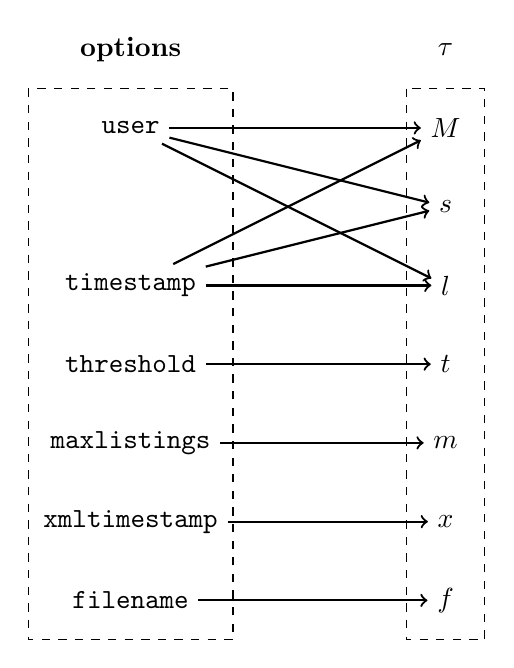
\begin{tikzpicture}
\node at (0,1) {\textbf{options}};
\node (u) at (0,0) {\verb+user+};
\node (time) at (0,-2) {\verb+timestamp+};
\node (thres) at (0,-3) {\verb+threshold+};
\node (max) at (0,-4) {\verb+maxlistings+};
\node (xml) at (0,-5) {\verb+xmltimestamp+};
\node (file) at (0,-6) {\verb+filename+};
\draw [dashed] (-1.3,.5) rectangle (1.3,-6.5);
\node at (4,1) {$\tau$};
\node (M) at (4,0) {$M$};
\node (s) at (4,-1) {$s$};
\node (l) at (4,-2) {$l$};
\node (t) at (4,-3) {$t$};
\node (m) at (4,-4) {$m$};
\node (x) at (4,-5) {$x$};
\node (f) at (4,-6) {$f$};
\draw [dashed] (3.5,.5) rectangle (4.5,-6.5);
\draw[->,thick] (u) -- (M);
\draw[->,thick] (u) -- (s);
\draw[->,thick] (u) -- (l);

\draw[->,thick] (time) -- (M);
\draw[->,thick] (time) -- (s);
\draw[->,thick] (time) -- (l);

\draw[->,thick] (thres) -- (t);

\draw[->,thick] (max) -- (m);
\draw[->,thick] (xml) -- (x);
\draw[->,thick] (file) -- (f);
\end{tikzpicture}
\end{center}
\caption{Dependency graph between the command line options and members of $\tau$}
\label{fig:depOR}
\end{figure}
Figure \ref{fig:depOR} illustrates which command line options are used for determining the members of the class. At first we show how do we determine $M$, $s$ and $l$. We use only the options \verb+user+ and \verb+timestamp+ for this. 

The first stage is selecting the data associated to the test we wish to evaluate. This process is illustrated on Figure \ref{fig:seltest}. 
\begin{figure}
\begin{center}
% Define block styles
\tikzstyle{decision} = [diamond, draw, 
    text width=4.5em, text badly centered, node distance=3cm, inner sep=0pt]
\tikzstyle{block} = [rectangle, draw, 
    text width=5em, text centered, rounded corners, minimum height=4em]
\tikzstyle{blockblue} = [rectangle, draw,fill=blue!20, 
    text width=5em, text centered, rounded corners, minimum height=4em]
\tikzstyle{blockred} = [rectangle, draw,fill=red!20, 
    text width=5em, text centered, rounded corners, minimum height=4em]
\tikzstyle{line} = [draw, -latex']
\tikzstyle{cloud} = [draw, ellipse,fill=gray!10, node distance=3cm,
    minimum height=2em]    
\begin{tikzpicture}[node distance = 2cm, auto]
    % Place nodes
    \node [block] (construct) {construct path to global user file};
    \node [cloud, left of=construct] (user) {\verb+user+};
    \node [blockblue, below of=construct] (parse) {parse global user file};
    \node [blockred, below of=parse, node distance=2.5cm] (listtests) {\verb+tests+:= list of all tests in global user file};
    \node [decision, below of=listtests] (decide) {\verb+ts==""?+};
    \node [cloud, left of=decide, node distance=4cm] (timestamp) {\verb+ts:=timestamp+}; 
    \node [block, below of=decide, node distance=4cm] (no) {find $i^{\ast}$ for which the timestamp attribute of \verb+tests[i]+ identical to \verb+ts+};
    \node [block, right of=no, node distance=4cm] (yes) {find $i^{\ast}$ for which the timestamp attribute of \verb+tests[i]+ is maximal};
    \node [block, below of=no, node distance=3.5cm] (test) {\verb+test:=+ $tests[i^{\ast}]$};
    % Draw edges
    \path [line] (construct) -- (parse);
    \path [line] (parse) -- (listtests);
    \path [line] (listtests) -- (decide);
    \path [line] (decide) -| node [near fstart] {yes} (yes);
    \path [line] (decide) -- node {no}(no);
    \path [line,dashed] (user) -- (construct);
    \path [line,dashed] (timestamp) -- (decide);
    \path [line] (no) -- (test);
    \path [line] (yes) |- (test);
\end{tikzpicture}
\end{center}
\caption{Selecting the relevant test data}
\label{fig:seltest}
\end{figure}
At the node with \colorbox{blue!20}{blue background} it might be possible that program execution halts without throwing an informative error due to the fact that no global user file can be found at the path constructed in the previous step of the program. See Issue \ref{iss:parseuser} for more details. At the node with \colorbox{red!20}{red background} it might be possible that the list we created is empty. If this is the case then it breask the program on the \emph{yes} branch of the decision node, however, it won't cause any trouble on the other branch (see Issue \ref{iss:emptytests}). If we specify a timestamp which can not be linked to any test then it won't break the program but the result wouldn't be of any use at all. One solution would be in this case to give a warning and jump to the other branch.  

The next stage goes on with the selected test and claculates the $M$, $s$ and $l$ members of $\tau$.  Figure \ref{fig:markings} shows how.
\begin{figure}
\begin{center}
% Define block styles
\tikzstyle{decision} = [diamond, draw, 
    text width=4.5em, text badly centered, node distance=3cm, inner sep=0pt]
\tikzstyle{block} = [rectangle, draw, 
    text width=5em, text centered, rounded corners, minimum height=4em]
\tikzstyle{blockblue} = [rectangle, draw,fill=blue!20, 
    text width=5em, text centered, rounded corners, minimum height=4em]
\tikzstyle{blockred} = [rectangle, draw,fill=red!20, 
    text width=5em, text centered, rounded corners, minimum height=4em]
\tikzstyle{line} = [draw, -latex']
\tikzstyle{cloud} = [draw, ellipse,fill=gray!10, node distance=3cm,
    minimum height=2em]    
\begin{tikzpicture}[node distance = 2cm, auto]
    % Place nodes
    \node [block] (subject) {$\tau@s=$ "subject" attribute of test};
    \node [block, right of=subject, node distance=2.5cm] (level) {$\tau@l=$ "level" attribute of test};
\end{tikzpicture}
\end{center}
\caption{Setting the $M$, $s$ and $l$ members of $\tau$.}
\label{fig:markings}
\end{figure}
\section{Teacher report}
\section{DT type teacher report}
\section{Issues}

\begin{enumerate}
\item\label{iss:parseuser}\textbf{Throw an informative error when the specified global user file can't be found} \colorbox{green}{Not critical} 

This issue is not critical because ``we know how to use the program''. The modifications we have to make to Figure \ref{fig:seltest} are shown in Figure \ref{fig:modseltest}.
\begin{figure}
\begin{center}
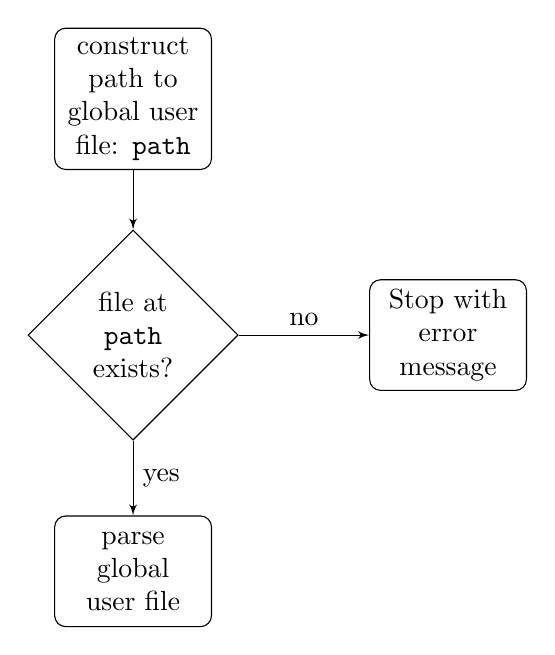
\begin{tikzpicture}[node distance = 2cm, auto]
% Define block styles
\tikzstyle{decision} = [diamond, draw, 
    text width=4.5em, text badly centered, node distance=3cm, inner sep=0pt]
\tikzstyle{block} = [rectangle, draw, 
    text width=5em, text centered, rounded corners, minimum height=4em]
\tikzstyle{line} = [draw, -latex']
    % Place nodes
    \node [block] (construct) {construct path to global user file: \verb+path+};
    \node [decision, below of=construct] (decide) {file at \verb+path+ exists?}; 
    \node [block, below of=decide, node distance=3cm] (parse) {parse global user file};
    \node [block, right of=decide, node distance=4cm] (no) {Stop with error message};
    \path [line] (construct) -- (decide);
    \path [line] (decide) -- node {yes} (parse);
    \path [line] (decide) -- node {no} (no);
\end{tikzpicture}
\end{center}
\caption{Error: User id not specified, non-existing user requested or user doesn't have a global user file.}
\label{fig:modseltest}
\end{figure}
\item\label{iss:emptytests}\textbf{A global user file doesn't containing any test entry breaks test selection when timestamp is not specified} \colorbox{green}{Not critical}

The cause of the problem is that one cannot call \verb+order+ or a \verb+NULL+ object in the function \verb+last+. But after all it would be better to check if the length of the tests object is equal to zero before the conditional statement and handle it not inside of the branches but before them. 

\item\label{iss:newtestsel}\textbf{Improving the test selection process} \colorbox{red}{Critical}




\end{enumerate}


\begin{itemize}
\item No example entry reported (must be verified)
\item rewrite of the script with while loop
\item Add more argument checking functionality.
%\item \label{iss:parseuser}\textbf{Throw an informative error when program is called without specifying the user argument:} fhjdhfd
jkfd
\end{itemize}

\section{Questions}
These are things to consider. They may or may not make sense. 
\begin{itemize}
\item New member of the result object: type=xml or tex.
\end{itemize}
\begin{enumerate}
\item\label{q:xmlstructure}\textbf{How about changing the structure of the result xml file?}
\begin{itemize}
\item \verb+<file>xmlresults.pdf</file>+ instead of \verb+<print file="xmlresult.pdf"/>+?
\item \verb+<subject>Lesen</subject>+ instead of \verb+<subject value="Lesen"/>+
\item \verb+<level>Schwer</level>+ instead of \verb+<level value="Schwer"/>+
\end{itemize}
\item\label{q:A1andA2}\textbf{Why is that something is listed in eval mode A1 and A2 as well?}

Here is an example:
\begin{verbatim}
./evalUser.R -u KFCG1 -t 50 -m 2 -T 2014_3_3_20_21_58 -x blahblah -f /tmp/xmlresult
\end{verbatim}
\item\label{q:defaults}\textbf{What should be the default value of the parameters?}
 
Current default values are listed in Table \ref{tab:op}
\begin{table}
\begin{center}
\begin{tabular}{rl}
\hline
option name & default value\\
\hline
threshold & 100\\
maxlistings & 3\\
timestamp & ''\\
xmltimestamp & ''\\
filename & ''\\
\hline
\end{tabular}
\end{center}
\caption{Default value of options}
\label{tab:op}
\end{table}

\end{enumerate}

\appendix

\section{ISO C99 / POSIX standard for 'strftime'}\label{app:posix}
\begin{tabular}{rp{14cm}} 
\%d & Day of the month as decimal number (01-31).\\
\%H & Hours as decimal number (00-23).  As a special exception times such as ‘24:00:00’ are accepted for input, since ISO 8601 allows these.\\
\%m & Month as decimal number (01-12).\\
\%M & Minute as decimal number (00-59).\\
\%S & Second as decimal number (00-61), allowing for up to two leap-seconds (but POSIX-compliant implementations will ignore leap seconds).\\
\%Y & Year with century.  Note that whereas there was no zero in the original Gregorian calendar, ISO 8601:2004 defines it to be valid (interpreted as 1BC): see \url{http://en.wikipedia.org/wiki/0_(year)}.  Note that the standard also says that years before 1582 in its calendar should only be used with agreement of the parties involved.
\end{tabular}
\end{document}
